\begin{figure}[h!]
    \centering
    \caption{Effects of a MW change on single family houses and condos rent per square foot (in dollars) for different definition of MW change event.}
    \scalebox{1}{
        \begin{subfigure}[b]{.5\linewidth}
            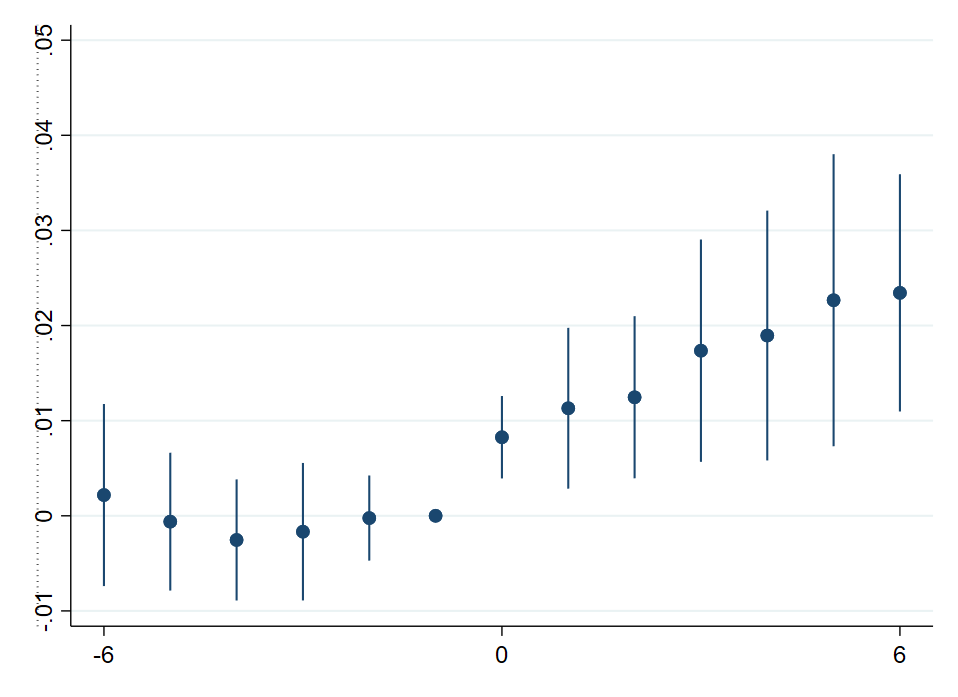
\includegraphics[width=\linewidth]{analysis/event_size_robustness/output/last_rentpsqft_sfcc_event025_w6.png}
            \caption{Mw changes of at least $\%0.25$}
        \end{subfigure}
        \quad 
        \begin{subfigure}[b]{.5\linewidth}
            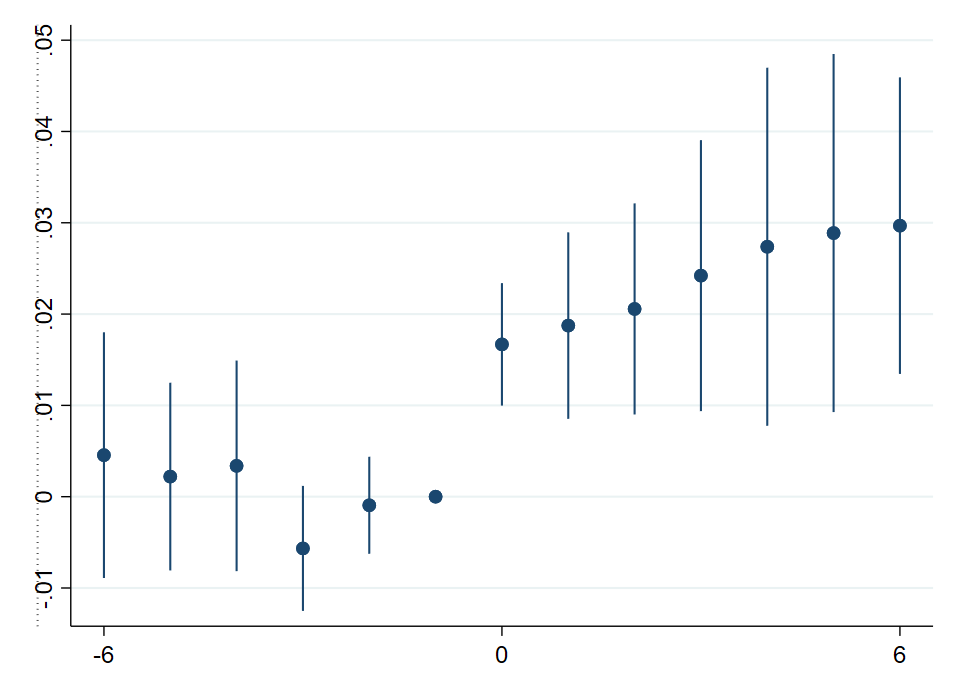
\includegraphics[width=\linewidth]{analysis/event_size_robustness/output/last_rentpsqft_sfcc_event075_w6.png}
            \caption{Mw changes of at least $\%0.75$}
        \end{subfigure}
    }
    \subcaption*{\textit{Note}: The figure shows the estimated $\hat{\delta}_{t+k}$ coefficients from the baseline specification (\autoref{eq:main_ziplevel}) for different events. In panel (a) we select all MW changes of at least $\$0.25$; in panel (b) we focus on all MW changes of at least $\$0.75$. For each zipcode, we  add the sum of unused events and county-level seasonality as additional controls ($X_{jt}$). Standard errors are clustered at the zipcode level.}
    \label{appfig:event_level_robustness6}
\end{figure}